% chapters/chapter3/3_2_lqr_step.tex
% !TeX root=../../main.tex

\section{ارزیابی \lr{LQR} در تنظیم نقطه ثابت}
\label{sec:lqr_step_analysis}

برای بررسی قابلیت‌ها و چالش‌های کنترل خطی در هدایت سیستم‌های زیرفعال، یک تنظیم‌گر خطی درجه دوم (\lr{LQR}) طراحی و عملکرد آن بر روی مدل فیزیکی غیرخطی در محیط \lr{Simscape} ارزیابی شده است. در این ساختار، طول کابل ثابت فرض شده ($l=l_0$) و فرمان کنترلی بر پایه فیدبک حالت به صورت $F=-KX$ تدوین شده است که در آن $X$ بردار حالت سیستم خطی‌شده است. تغذیه مستقیم خطای موقعیت به عنوان مرجع ورودی پله، سیستم را در شرایط عملیاتی متفاوتی قرار می‌دهد که در ادامه تحت دو سناریوی جابه‌جایی $0.5$ متر و $5$ متر تحلیل می‌شود.

\subsection{مانور کوتاه‌برد}

در سناریوی نخست، کالسکه در موقعیت اولیه $-0.5$ متر قرار گرفته و هدف، هدایت آن به مبدأ مختصات است. نتایج شبیه‌سازی در شکل~\ref{fig:lqr_step_05_results} نشان می‌دهد که کنترل‌کننده خطی کالسکه را با رفتاری میرا به نقطه هدف هدایت می‌کند. دامنه انحراف آونگ در بیشینه خود به حدود $0.25$ رادیان می‌رسد که به مرز فیزیکی $15^\circ$، معادل تقریباً $0.26$ رادیان، نزدیک است؛ با این حال از این مرز فراتر نمی‌رود.

پایداری مشاهده‌شده در این مانور با محدود بودن خطای اولیه و باقی ماندن پاسخ در ناحیه‌ای نسبتاً نزدیک به نقطه تعادل سازگار است. همان‌گونه که پروفایل نیروی کنترلی در شکل~\ref{fig:lqr_step_05_force} نشان می‌دهد، بیشینه فرمان نیرویی در لحظه آغازین حدود $15.5\,\mathrm{N}$ است. این مقدار کمتر از کران فیزیکی واقعی سیستم، یعنی $50\,\mathrm{N}$، است. خطوط چین‌دار موجود در شکل صرفاً برای مقیاس‌بندی و نمایش خواناتر سیگنال رسم شده‌اند و نشان‌دهنده قید واقعی عملگر نیستند. در این شرایط، دامنه نوسان آونگ در محدوده‌ای باقی می‌ماند که تقریب خطی $\sin\theta\approx\theta$ همچنان با تقریب قابل‌قبولی قابل استفاده است.

\begin{figure}[htbp]
    \centering
    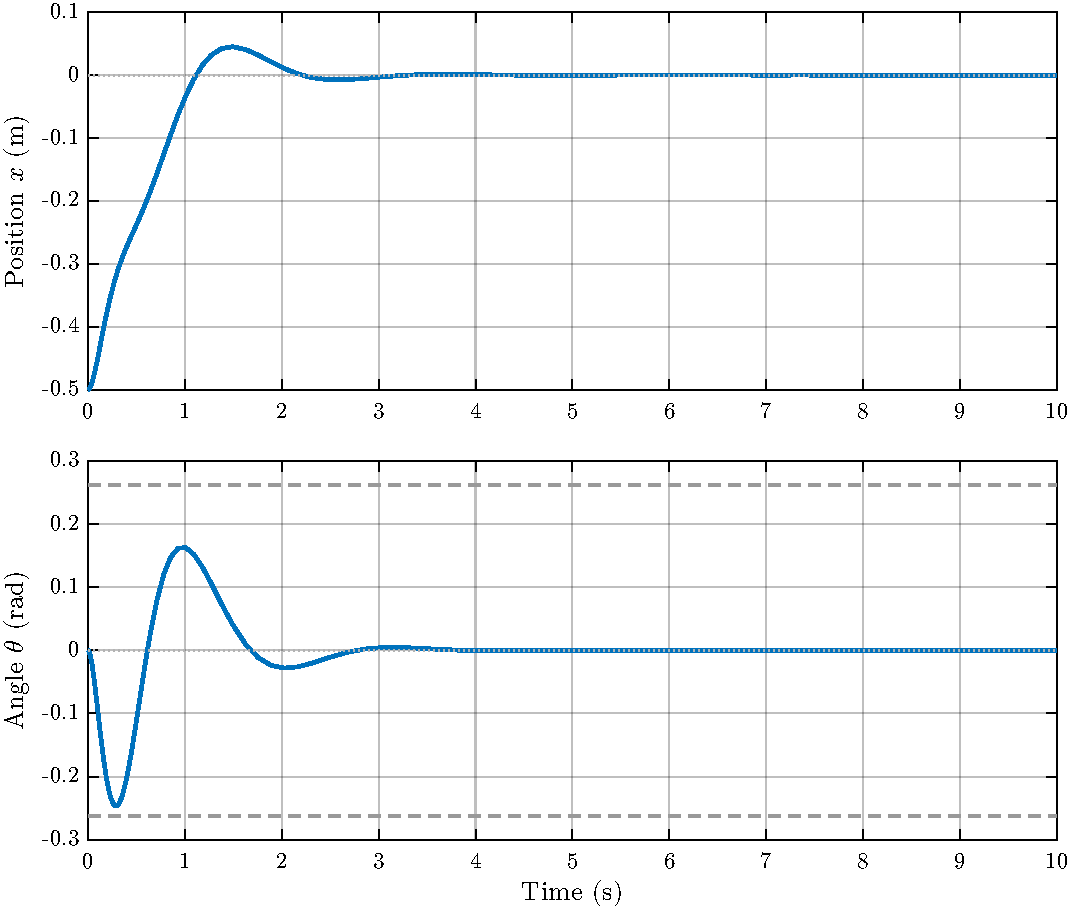
\includegraphics[width=0.88\textwidth]{images/1_LQR_Step/LQR_x_theta.pdf}
    \caption{\rl{پاسخ زمانی موقعیت کالسکه و زاویه آونگ برای جابه‌جایی $0.5$ متر.}}
    \label{fig:lqr_step_05_results}
\end{figure}

\begin{figure}[htbp]
    \centering
    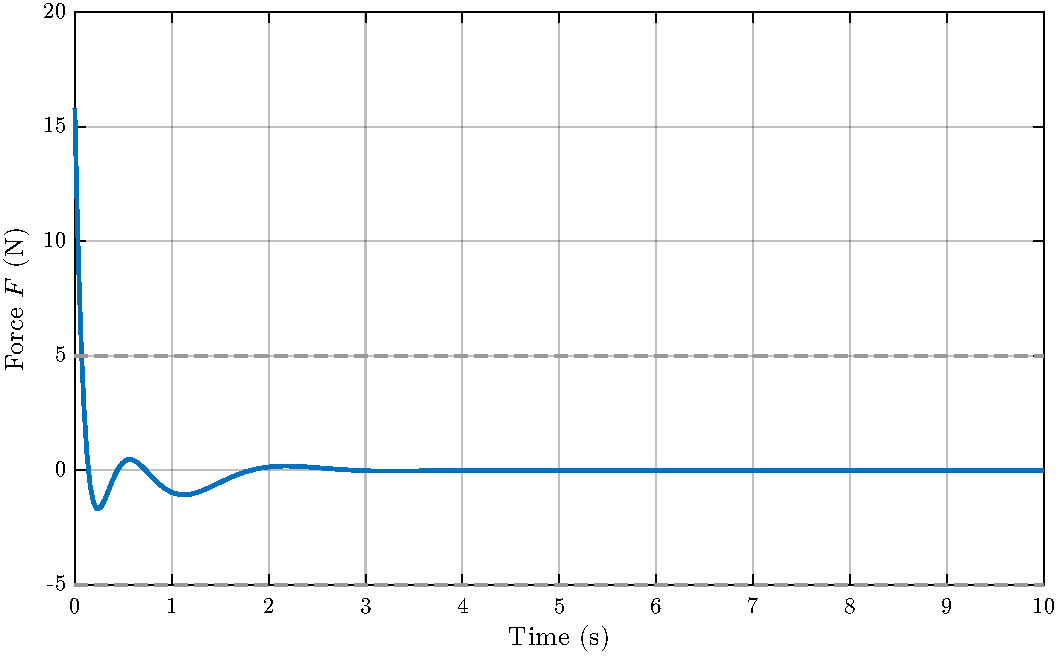
\includegraphics[width=0.88\textwidth]{images/1_LQR_Step/LQR_F.pdf}
    \caption{\rl{فرمان نیروی کنترلی اعمال‌شده به کالسکه برای جابه‌جایی $0.5$ متر.}}
    \label{fig:lqr_step_05_force}
\end{figure}

\subsection{مانور بلندبرد}

با افزایش خطای اولیه به $5$ متر، رفتار دینامیکی سیستم محدودیت‌های ساختاری این رویکرد خطی را آشکار می‌سازد. همان‌گونه که در شکل~\ref{fig:lqr_step_5_force} مشاهده می‌شود، فرمان اولیه نیروی کنترلی به حدود $160\,\mathrm{N}$ می‌رسد؛ مقداری که از کران فیزیکی واقعی عملگر، یعنی $50\,\mathrm{N}$، فراتر می‌رود. این نتیجه نشان می‌دهد که قانون \lr{LQR}، که بر اساس مدل خطی‌شده طراحی شده است، در این شرایط بدون درنظرگرفتن محدودیت عملگر فرمانی خارج از محدوده مجاز تولید می‌کند.

پیامد این تحریک شدید در شکل~\ref{fig:lqr_step_5_results} مشاهده می‌شود. زاویه آونگ به سرعت از ناحیه کوچک اطراف نقطه تعادل خارج شده و پس از یک چرخش کامل در نزدیکی $\theta\approx-6.28$ رادیان، معادل $-2\pi$، قرار می‌گیرد. از دیدگاه فیزیکی، این زاویه با وضعیت آویزان آونگ هم‌ارز است؛ با این حال، مدل خطی‌شده حول $\theta=0$، چنین تغییر زاویه بزرگی را در همان چارچوب محلی تفسیر می‌کند و نمی‌تواند هم‌ارزی فیزیکی زوایای تکرارشونده را بازنمایی کند.

در نتیجه، سیستم به یک تعادل نهایی نامطلوب وارد می‌شود که در آن کالسکه در موقعیتی حدود $x\approx-3.5$ متر متوقف می‌شود. با صفر شدن سرعت‌ها و نیروی کنترلی در حالت ماندگار، رابطه
\[
    F=-k_1x_{\mathrm{ss}}-k_3\theta_{\mathrm{ss}}=0
\]
نشان می‌دهد که موقعیت نهایی کالسکه می‌تواند تحت تأثیر مؤلفه زاویه‌ای فیدبک قرار گیرد. از این رو، توقف کالسکه در فاصله قابل توجهی از نقطه هدف را می‌توان پیامد مستقیم خروج سیستم از ناحیه‌ای دانست که مدل خطی‌شده برای آن اعتبار دارد.

\begin{figure}[htbp]
    \centering
    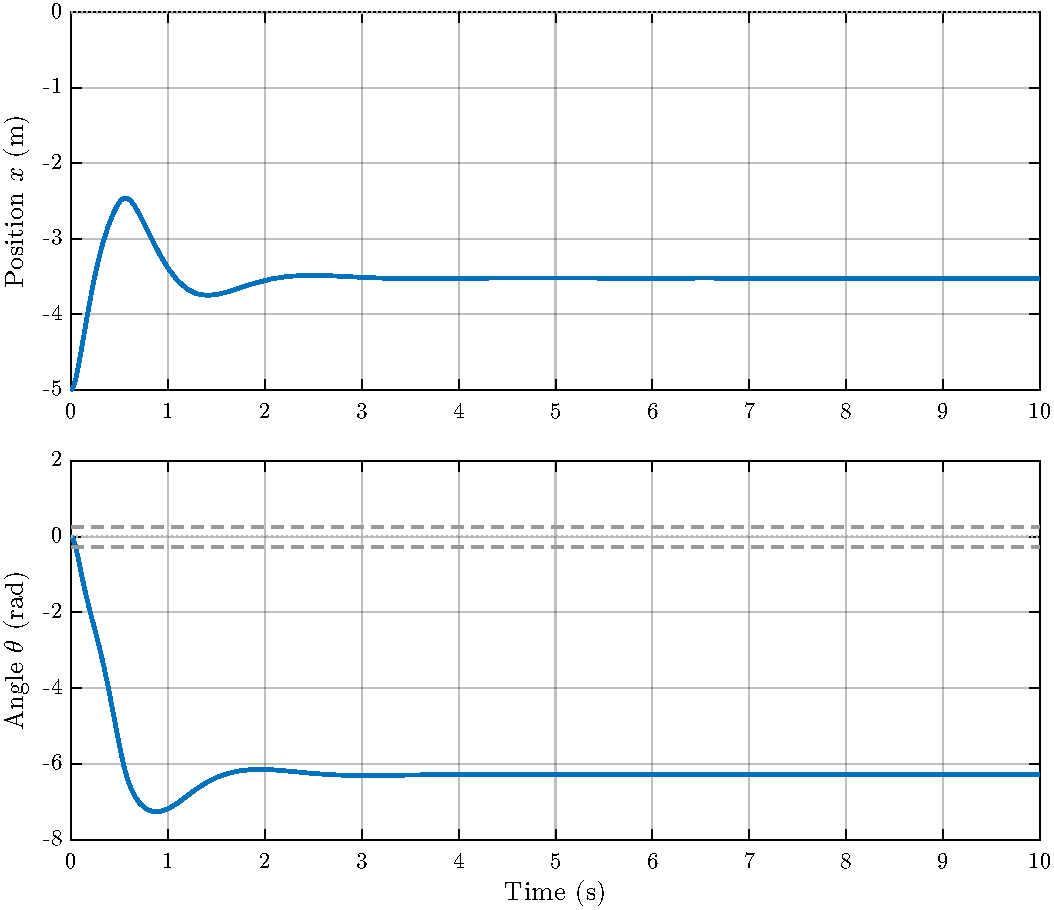
\includegraphics[width=0.88\textwidth]{images/1_LQR_Step/LQR_x_theta_5.pdf}
    \caption{\rl{پاسخ زمانی سیستم در جابه‌جایی $5$ متر و خروج آونگ از محدوده عملکرد خطی.}}
    \label{fig:lqr_step_5_results}
\end{figure}

\begin{figure}[htbp]
    \centering
    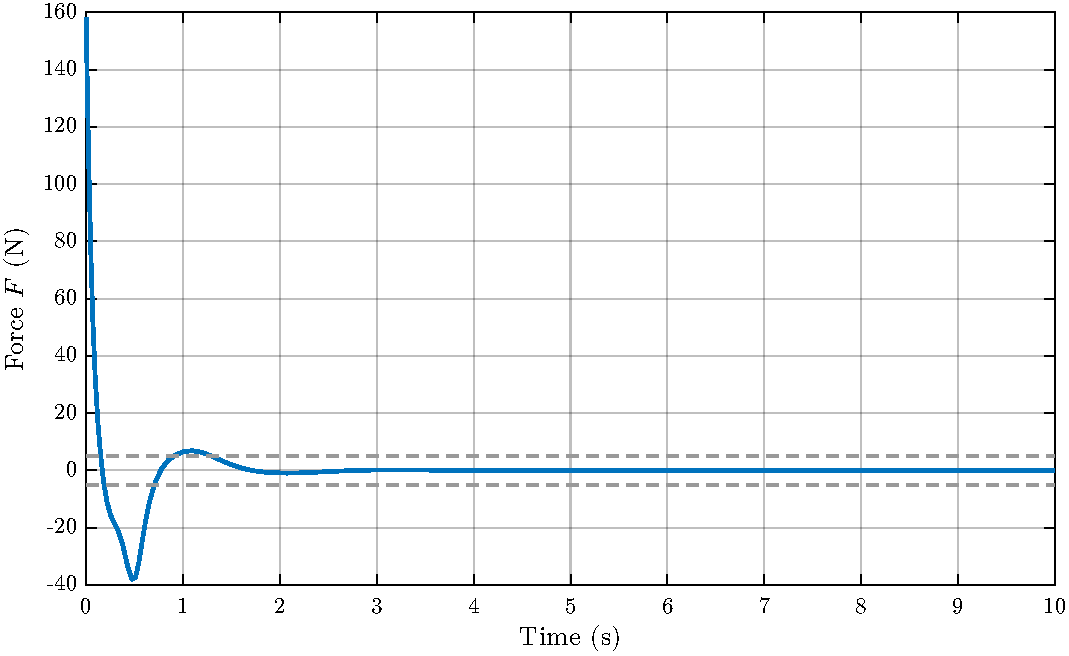
\includegraphics[width=0.88\textwidth]{images/1_LQR_Step/LQR_F_5.pdf}
    \caption{\rl{فرمان اولیه نیروی کنترلی برای جابه‌جایی $5$ متر و تجاوز آن از کران فیزیکی $50\,\mathrm{N}$.}}
    \label{fig:lqr_step_5_force}
\end{figure}

\subsection{جمع‌بندی محدودیت \lr{LQR} در تحریک پله}

مقایسه پاسخ سیستم در دو مانور نشان می‌دهد که عملکرد \lr{LQR} به اعتبار محلی مدل خطی وابسته است. در مانور $0.5$ متری، خطای اولیه محدود و فرمان نیرویی در محدوده مجاز باقی می‌ماند و پاسخ آونگ نیز در نزدیکی نقطه تعادل حفظ می‌شود. در مقابل، افزایش فاصله هدف به $5$ متر باعث تولید فرمانی فراتر از کران فیزیکی عملگر و خروج سریع آونگ از ناحیه خطی می‌شود. بنابراین، برای مدیریت مانورهای بلندبرد در این چارچوب، اعمال مستقیم خطای بزرگ به عنوان ورودی کنترل مناسب نیست و استفاده از یک مسیر مرجع هموار و محدود، زمینه منطقی‌تری برای ادامه ارزیابی فراهم می‌کند.
